\documentclass[conference]{IEEEtran}
\IEEEoverridecommandlockouts
\usepackage{cite}
\usepackage{amsmath,amssymb}
\usepackage{graphicx}
\usepackage{array}
\usepackage{tikz}
\usetikzlibrary{positioning,arrows.meta}

\begin{document}

\title{Temporal Matching of CCTV, GPS and Written Evidence for Forensic Event Reconstruction\\
{\large A Study of Time Uncertainty and Evidence Provenance}
\thanks{Research Methodology -- Phase I Research Progress Report, submitted to Dr. Tanupriya Choudhury.}
}

\author{
\IEEEauthorblockN{Vansh Rana}
\IEEEauthorblockA{SAP ID: 590017823}
\and
\IEEEauthorblockN{Anirudh Singh Aswal}
\IEEEauthorblockA{SAP ID: 590017310}
\and
\IEEEauthorblockN{Hardik Trivedi}
\IEEEauthorblockA{SAP ID: 590016152}
\and
\IEEEauthorblockN{Yash Shrivastava}
\IEEEauthorblockA{SAP ID: 590011391}
}

\maketitle

\begin{abstract}
In an investigation there can be CCTV videos, location records and written statements about the same incident, but these sources do not always agree on the time. A camera can have a wrong clock, a GPS record can have some measurement error, and a witness may just say that something happened ``around'' some time. In this paper we look at whether showing time as an interval (a range) instead of one exact value helps in matching the records from these sources. Our plan is to first process each source on its own and then compare the records using time, location and the event they describe. Every match will keep a link back to the original video frame, GPS record or text line. We will test the method on controlled scenarios and compare it with simple timestamp based matching. The experiments are not done yet, so this report only explains the proposed study.
\end{abstract}

\begin{IEEEkeywords}
digital forensics, event reconstruction, CCTV, GPS trajectories, temporal uncertainty, evidence provenance
\end{IEEEkeywords}

\section{Introduction}
A CCTV video, a phone location trace and an incident report can each show a different part of the same event. The hard part is to decide if these records are really about the same event or not. A camera timestamp can be some minutes ahead of the real time. A GPS point tells where a device was, but it does not tell who was carrying it. A written statement may give only a rough time, or it may describe an action in a different way than what is seen in the video. So if we match records just because their timestamps are close, we can end up linking things that are not actually related.

Some earlier studies have worked on parts of this problem. Edelman and Bijhold synchronized CCTV streams and showed tracked movements in a 3D model, and they used GPS recordings from test participants to check the reconstructed movements \cite{b1}. Kraus et al. made ISRA-4D, which lets investigators look at video and image material inside a shared 3D scene \cite{b2}. These works show that video can be used for spatial and temporal reconstruction. But they do not explain how a video track should be matched with a separate GPS trajectory and with an event taken from a written statement, when the time of each source is not certain.

So the main question of our study is: Does showing the time uncertainty of each source improve the accuracy of matching events across sources, compared to matching records only by timestamp? The output we want is a timeline of possible events, where each match has links to the records behind it. It is not meant to identify a person or to decide who is legally responsible.

\section{Related Work}
This is only a first review, not a full systematic review of all papers in this field. We found the papers by searching for CCTV based reconstruction, digital forensic timelines, GPS trajectories, multimodal event detection, timestamp interpretation and evidence provenance. We checked publisher records and full texts wherever we had access.

\subsection{Video and Visual Evidence}
Edelman and Bijhold \cite{b1} is the closest work to the video part of our proposal. They synchronized many CCTV streams and rebuilt the movement in a 3D model. GPS data was recorded by test participants and used as ground truth to check the tracks. This is different from our idea, where an independent GPS feed is an input that has to be linked with the CCTV observations. Kraus et al. \cite{b2} built an interactive 4D scene reconstruction system to examine video and images from different cameras, and its focus is on looking at visual evidence in space and time. Milliet et al. \cite{b3} explain a step by step way of using trace images in an investigation: information is collected, organized, used to build a reconstruction and then evaluated. Schindler et al. \cite{b4} present a video forensic platform for analysing material collected after a terrorist attack. All these papers show that multi camera analysis and visual reconstruction are not new problems.

\subsection{Time Interpretation and Forensic Timelines}
Weyermann, Vanini and Souvignet \cite{b5} talk about three ways to place physical and digital traces in time: time tags, time dynamics and relative sequences. Their framework is useful for us because it does not assume that a timestamp is always correct. Vanini et al. \cite{b6} look at clock errors using the idea of time anchors, which are events that help to check if a system clock was correct or not. In digital forensics, Hargreaves and Patterson \cite{b7} show how low level computer events can be joined to find higher level events while still keeping the source records. Breitinger et al. \cite{b8} review timeline based event reconstruction and point out problems that are still open, like uncertainty, interpretation and inferring events from digital artifacts.

\subsection{Evidence Fusion and Provenance}
Mondal et al. \cite{b9} classify multimodal event detection methods based on where the fusion happens, that is at feature level, representation level or decision level. Digital Stratigraphy \cite{b10} is quite close to our study since it combines digital logs, geospatial traces, criminology records and excavation data in a time based framework. Its dataset is only available on request from the authors, so we cannot use it as a free benchmark. ForenThings \cite{b11} reconstructs incidents in smart environments by linking events from IoT devices and apps, and it also keeps data provenance. VeriScene \cite{b12}, a 2026 preprint, works with forensic photos and witness statements and focuses on traceable claims and conflicting accounts. Because of these studies, we cannot say that evidence fusion, event timelines or provenance graphs are new contributions by themselves.

\section{Research Gap and Questions}
The work we reviewed covers multi camera reconstruction, forensic time interpretation, digital timelines and some types of evidence fusion. Our study is more narrow. We want to test if time intervals made for each source improve the matching of: (i) events seen in continuous CCTV footage, (ii) segments from independent GPS trajectories, and (iii) events taken from written incident accounts. We will focus on cases where timestamps have known offsets, where some records are missing, or where two sources do not agree. From what we have read so far, we did not find a directly comparable evaluation of this exact setup. This is a working research gap, we are not claiming that no similar system exists.

Our study will try to answer three questions:
\begin{enumerate}
\item Does using interval based time reduce wrong matches when the source clocks have known offsets?
\item Does adding location and event description information give better matching than using time only?
\item Can the final timeline show which source records support or contradict each possible event?
\end{enumerate}

\section{Research Objectives}
We have planned the work around four objectives:
\begin{enumerate}
\item To study existing methods for video tracking, GPS trajectory processing, temporal information extraction and forensic event reconstruction.
\item To define a common format for storing observations from video, GPS and written accounts, without losing the original source information.
\item To develop a matching method that uses time, location and event description, and keeps uncertain matches open for review.
\item To compare our method with timestamp based methods using controlled scenarios where the event sequence and source links are already known.
\end{enumerate}

\section{Scope and Assumptions}
Our prototype will take three types of input: CCTV style video, GPS traces with timestamps and short incident narratives. We will not use face recognition. If a person is seen in a video and a GPS device is nearby, we will treat them as two separate observations unless there is some other evidence that links them. This way being close in location is not taken as proof of identity. Video processing will give track segments and visible event cues, GPS processing will arrange coordinate records into movement segments, and text processing will pull out entities, actions and time expressions. All these outputs will be treated as observations that can have errors, not as confirmed facts.

The main end to end testing will use controlled scenarios that we will prepare for this study. Public datasets can be used to test single components, but datasets collected separately will not be shown as if they describe the same incident. If we use any real CCTV footage or personal location data, we will need permission and proper ethical review.

\section{Proposed Methodology}

\subsection{Processing the Three Sources}
Each source will be processed separately first and then the outputs will be compared. For CCTV, the system will store track segments, frame references, camera IDs and visible event cues. For GPS, it will keep coordinate sequences, device timestamps and the accuracy information that comes with the records. For written accounts, it will find the people or objects mentioned, the action described and any time expression. For example, ``at about 8 pm'' should stay as an approximate time and not be changed into one exact timestamp. Table~\ref{tab:sources} shows what we will take from each source.

\begin{table}[htbp]
\caption{Information to be Extracted from Each Source}
\label{tab:sources}
\centering
\renewcommand{\arraystretch}{1.2}
\begin{tabular}{|p{0.17\columnwidth}|p{0.36\columnwidth}|p{0.32\columnwidth}|}
\hline
Source & Processing Output & Purpose in the Study \\
\hline
CCTV video & Track segment, frame range, camera ID and visible event cue & Record where and when an action is visible \\
\hline
GPS trace & Coordinate sequence, device time and reported location accuracy & Describe the recorded movement of a device \\
\hline
Incident account & Entity, action and exact or approximate time expression & Represent the event described in writing \\
\hline
\end{tabular}
\end{table}

\subsection{Common Observation Record}
All the outputs will be saved in one common record. It will have an observation ID, source ID, original timestamp, estimated time interval, location or area (if available), event description, extraction confidence and a reference to the original evidence. This reference can be a video frame, a GPS row or the sentence from which the text observation was taken. We will keep extraction confidence separate from source reliability. For example, a model can be very sure that a person is visible in a frame, but that does not mean the camera clock is correct.

\subsection{Time Correction and Candidate Matching}
The first step is to bring all recorded times to one common reference where we have enough information. Known time zone differences and measured clock offsets will be corrected. If the real time cannot be narrowed down to one value, the system will keep a time interval. We will also record how each interval was made, so the investigator can see if it came from a measured clock offset, a GPS accuracy field or a rough time written in a statement.

After this, the system will compare possible matches. It will check if their time intervals overlap or are close, if their locations make sense together, and if their event or action descriptions can be about the same thing. A match will not be accepted just because two timestamps are close. The comparison rules and weights will be set using development scenarios and will not be changed for the final test set. Observations that do not meet the matching conditions will stay unmatched.

\subsection{Event Graph and Timeline}
The system will keep the source observations separate from the event hypotheses made from them. A graph will store links like ``supports'', ``contradicts'' and ``used to infer''. This is important because two records may not agree, and the system should keep both of them instead of quietly picking one. The timeline will put events in order when the time information allows it. Where time intervals overlap, the system will show that the order is not certain.

\subsection{Methodology Flowchart}
Fig.~\ref{fig:flow} shows the planned steps, from processing each source to making a timeline for review.

\begin{figure}[htbp]
\centering
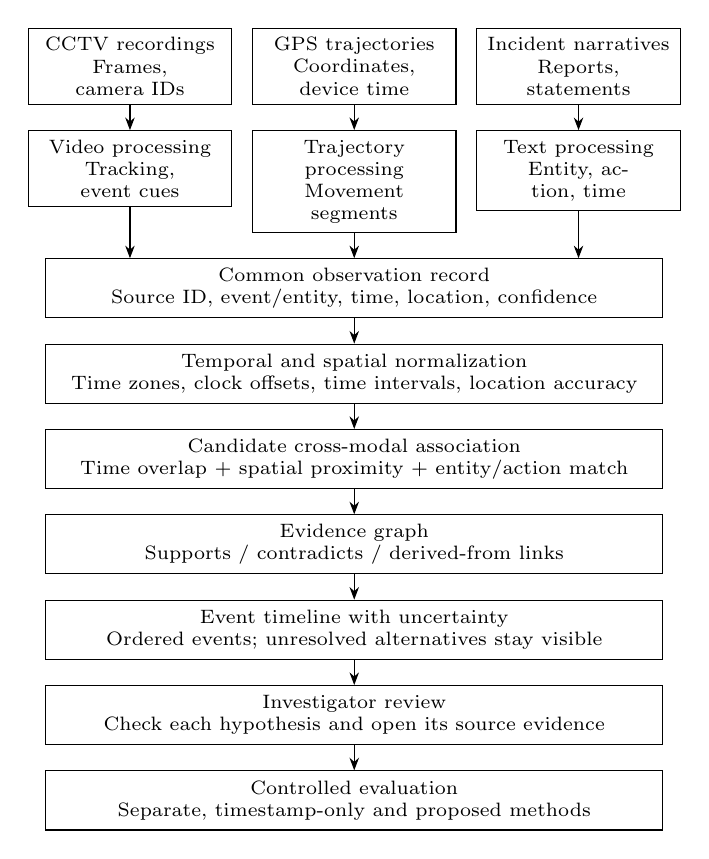
\begin{tikzpicture}[
  font=\scriptsize,
  box/.style={draw, rectangle, align=center, minimum height=0.75cm, text width=2.35cm},
  wide/.style={draw, rectangle, align=center, minimum height=0.75cm, text width=7.6cm},
  arr/.style={-{Stealth[length=1.6mm]}},
  node distance=0.32cm and 0.25cm
]
\node[box] (gps) {GPS trajectories\\ Coordinates, device time};
\node[box, left=of gps] (cctv) {CCTV recordings\\ Frames, camera IDs};
\node[box, right=of gps] (txt) {Incident narratives\\ Reports, statements};

\node[box, below=of cctv] (vp) {Video processing\\ Tracking, event cues};
\node[box, below=of gps] (tp) {Trajectory processing\\ Movement segments};
\node[box, below=of txt] (xp) {Text processing\\ Entity, action, time};

\node[wide, below=of tp] (rec) {Common observation record\\ Source ID, event/entity, time, location, confidence};
\node[wide, below=of rec] (norm) {Temporal and spatial normalization\\ Time zones, clock offsets, time intervals, location accuracy};
\node[wide, below=of norm] (assoc) {Candidate cross-modal association\\ Time overlap + spatial proximity + entity/action match};
\node[wide, below=of assoc] (graph) {Evidence graph\\ Supports / contradicts / derived-from links};
\node[wide, below=of graph] (time) {Event timeline with uncertainty\\ Ordered events; unresolved alternatives stay visible};
\node[wide, below=of time] (rev) {Investigator review\\ Check each hypothesis and open its source evidence};
\node[wide, below=of rev] (eval) {Controlled evaluation\\ Separate, timestamp-only and proposed methods};

\draw[arr] (cctv) -- (vp);
\draw[arr] (gps) -- (tp);
\draw[arr] (txt) -- (xp);
\draw[arr] (vp.south) -- (vp.south |- rec.north);
\draw[arr] (tp) -- (rec);
\draw[arr] (xp.south) -- (xp.south |- rec.north);
\draw[arr] (rec) -- (norm);
\draw[arr] (norm) -- (assoc);
\draw[arr] (assoc) -- (graph);
\draw[arr] (graph) -- (time);
\draw[arr] (time) -- (rev);
\draw[arr] (rev) -- (eval);
\end{tikzpicture}
\caption{Planned processing and evaluation workflow.}
\label{fig:flow}
\end{figure}

The output will let an investigator open the records linked to a possible event. It is meant as a way to organize information for review, not as an automatic decision about what happened.

\section{Experimental Design and Evaluation}

\subsection{Data Sources}
The experiments will be done at two levels. First, public datasets will be used only to check single components. MOT16 has annotated pedestrian tracking sequences and can be used to check the video tracking output \cite{b13}. GeoLife has GPS trajectories and can be used to test trajectory processing \cite{b14}. These two datasets are not related to each other and do not describe the same incidents. Second, controlled scenarios will be used for the main end to end test. Each scenario will have a scripted sequence of events, CCTV style clips, simulated GPS traces and short written accounts. The links between observations and the known events will be marked before testing. Table~\ref{tab:data} lists the planned datasets.

\begin{table}[htbp]
\caption{Planned Datasets and Their Intended Use}
\label{tab:data}
\centering
\renewcommand{\arraystretch}{1.2}
\begin{tabular}{|p{0.18\columnwidth}|p{0.33\columnwidth}|p{0.34\columnwidth}|}
\hline
Data Source & What it Contains & Use and Limitation \\
\hline
MOT16 & Pedestrian videos with tracking annotations & Check the tracking part; not a forensic incident dataset \\
\hline
GeoLife & GPS trajectories collected from many users & Check trajectory processing; not linked to MOT16 \\
\hline
Controlled scenarios & Scripted video, simulated GPS and annotated narratives & Main test set, with known event order and source links \\
\hline
\end{tabular}
\end{table}

\subsection{Comparison Methods and Test Conditions}
We will compare three setups on the same controlled scenarios:
\begin{enumerate}
\item Separate processing: each source is analysed on its own, with no matching across sources.
\item Timestamp matching: observations are linked using an exact timestamp or a fixed time window.
\item Proposed method: observations are compared using time intervals, location and event description.
\end{enumerate}

The scenarios will have camera and GPS clock offsets, missing observations, location noise and conflicting details in the narratives. The offset values and the correct event links will be written down in advance. Parameters will be chosen on development scenarios and then kept fixed during testing.

\subsection{Evaluation Measures}
Association precision, recall and F1-score will show if observations are linked to the right event. Temporal interval coverage will measure how often the known event time falls inside the interval given by the system. We will also report the width of the interval, so that very wide estimates are not counted as good automatically. Event ordering accuracy will be calculated for events whose real order is known. Conflict detection precision and recall will measure how often the records we made inconsistent on purpose are flagged. Traceability coverage will measure how many event hypotheses still have links to their source observations. No results are given here because the experiments are still proposed work.

\subsection{Limitations and Planned Work}
Controlled scenarios let us add known clock offsets and missing records, but they cannot show how the method will work in a real investigation. MOT16 and GeoLife are useful only for testing separate components, and neither of them has synchronized video, GPS and incident narratives. So the first stage of our work will be to prepare the observation format and the controlled scenarios, and then compare the three setups. Even if the method works well on these tests, it will still need to be tested on real world data with proper permission.

\section{Expected Contribution}
We expect this study to give a tested comparison between timestamp only matching and a method that shows the uncertainty in source times. It will also show which kinds of missing or conflicting information make the method give wrong matches. What we want to contribute is a small prototype that can be reviewed, along with an evaluation of its limits, and not a complete crime scene investigation system.

\begin{thebibliography}{00}
\bibitem{b1} G. Edelman and J. Bijhold, ``Tracking people and cars using 3D modeling and CCTV,'' \emph{Forensic Sci. Int.}, vol. 202, no. 1--3, pp. 26--35, 2010, doi: 10.1016/j.forsciint.2010.04.021.
\bibitem{b2} M. Kraus et al., ``Toward mass video data analysis: Interactive and immersive 4D scene reconstruction,'' \emph{Sensors}, vol. 20, no. 18, Art. no. 5426, 2020, doi: 10.3390/s20185426.
\bibitem{b3} Q. Milliet, O. Del\'emont, E. Sapin, and P. Margot, ``A methodology to event reconstruction from trace images,'' \emph{Sci. Justice}, vol. 55, no. 2, pp. 107--117, 2015, doi: 10.1016/j.scijus.2015.02.001.
\bibitem{b4} A. Schindler, A. Lindley, A. Naghibzadeh-Jalali, M. Boyer, S. Gordea, and R. C. King, ``Multi-modal video forensic platform for investigating post-terrorist attack scenarios,'' in \emph{Proc. 11th ACM Multimedia Syst. Conf.}, 2020, pp. 365--368, doi: 10.1145/3339825.3393585.
\bibitem{b5} C. Weyermann, C. Vanini, and T. R. Souvignet, ``A common framework to situate digital and physical traces in time,'' \emph{Forensic Sci. Int.}, vol. 360, Art. no. 112020, 2024, doi: 10.1016/j.forsciint.2024.112020.
\bibitem{b6} C. Vanini, C. J. Hargreaves, H. van Beek, and F. Breitinger, ``Was the clock correct? Exploring timestamp interpretation through time anchors for digital forensic event reconstruction,'' \emph{Forensic Sci. Int.: Digit. Investig.}, vol. 49, Art. no. 301759, 2024, doi: 10.1016/j.fsidi.2024.301759.
\bibitem{b7} C. Hargreaves and J. Patterson, ``An automated timeline reconstruction approach for digital forensic investigations,'' \emph{Digit. Investig.}, vol. 9, suppl., pp. S69--S79, 2012, doi: 10.1016/j.diin.2012.05.006.
\bibitem{b8} F. Breitinger, H. Studiawan, and C. Hargreaves, ``SoK: Timeline based event reconstruction for digital forensics: Terminology, methodology, and current challenges,'' \emph{Forensic Sci. Int.: Digit. Investig.}, vol. 53, Art. no. 301932, 2025, doi: 10.1016/j.fsidi.2025.301932.
\bibitem{b9} M. Mondal, M. Khayati, H.-A. Sandlin, and P. Cudr\'e-Mauroux, ``A survey of multimodal event detection based on data fusion,'' \emph{VLDB J.}, vol. 34, Art. no. 9, 2025, doi: 10.1007/s00778-024-00878-5.
\bibitem{b10} R. Rawat, H. Rawat, M. Ingle, A. Rawat, A. Rajavat, and A. Dibouliya, ``Digital stratigraphy---A pattern analysis framework integrating computer forensics, criminology, and forensic archaeology for crime scene investigation,'' \emph{Forensic Sci.}, vol. 5, no. 4, Art. no. 48, 2025, doi: 10.3390/forensicsci5040048.
\bibitem{b11} E. Khodayarseresht, S. Smolyakova, L.-Y. Zhao, A. Mansouri, S. Majumdar, and M. Conti, ``ForenThings: An interactive framework for crime scene reconstruction in IoT forensics,'' \emph{ACM Trans. Internet Things}, vol. 7, no. 1, 2026, doi: 10.1145/3772067.
\bibitem{b12} K. C. Fu, Y. Zheng, Z. K. Yeong, and K.-Y. Lam, ``VeriScene: Reconstructing crime scenes from legal evidence via world-model agent,'' 2026, \emph{arXiv:2609.08342}.
\bibitem{b13} A. Milan, L. Leal-Taix\'e, I. Reid, S. Roth, and K. Schindler, ``MOT16: A benchmark for multi-object tracking,'' 2016, \emph{arXiv:1603.00831}.
\bibitem{b14} Y. Zheng, L. Zhang, X. Xie, and W.-Y. Ma, ``Mining interesting locations and travel sequences from GPS trajectories,'' in \emph{Proc. 18th Int. Conf. World Wide Web}, 2009, pp. 791--800, doi: 10.1145/1526709.1526816.
\end{thebibliography}

\end{document}
